\documentclass[compress]{beamer}
\useoutertheme[footline=authortitle,subsection=false]{miniframes}
\setbeamertemplate{navigation symbols}{}

\definecolor{vertmoyen}{HTML}{A9CB60}
\definecolor{vertclair}{HTML}{D3F192}
\definecolor{vertfonce}{HTML}{347003}
\definecolor{deletecol}{HTML}{3B8A13}
\definecolor{addcolor} {HTML}{9E0270}

\usecolortheme[named=vertfonce]{structure}

\setbeamercolor{section in head/foot}{fg=vertfonce,bg=vertmoyen}
\setbeamercolor{author in head/foot}{fg=white}
\setbeamercolor{titlelike}{bg=vertclair}
\setbeamertemplate{mini frame in other subsection}[default][0!white!100]
\setbeamertemplate{section in head/foot shaded}[default][0!white!100]


\usepackage[utf8]{inputenc}
\usepackage[T1]{fontenc}

\usepackage{kpfonts}

\usepackage{amsmath,bussproofs}

\usepackage{graphics,booktabs,array}

\title{Combining RecyclePivotsWithIntersection and LowerUnits}
\author[Joseph Boudou]{Joseph Boudou, Bruno Woltzenlogel Paleo}

\def\fCenter{\mbox{\large\ $\vdash$\ }}
\newcommand{\InfDesc}[1]{\RightLabel{\tiny $(#1)$}}

\newcommand{\siecle}[1]{\textsc{\romannumeral #1}\textsuperscript{e}~siècle}

\newenvironment{subpart}[1]
{ \begin{block}{#1}
  \begin{itemize}
}{
  \end{itemize}
  \end{block}
}

\usepackage{tikz}
\usetikzlibrary{arrows,matrix,positioning}

\tikzstyle{proof edge}=[thick,cap=round]
\tikzstyle{deleted edge}=[proof edge, dashed, color=deletecol]

\newcommand{\proofnode}[3][]{
  \node [anchor=mid, #1] (#2) {#3}
}

\newcommand{\rootnode}[1][]{
  \proofnode[#1]{root}{$\bot$}
}

\newcommand{\drawchildren}[3]{
  \draw [proof edge] (#1) -- (#2);
  \draw [proof edge] (#1) -- (#3)
}

\newcommand{\addchildren}[5]{
  \proofnode[above left  of=#1]{#2}{#3};
  \proofnode[above right of=#1]{#4}{#5}
}

\newcommand{\withchildren}[5]{
  \addchildren{#1}{#2}{#3}{#4}{#5};
  \drawchildren{#1}{#2}{#4}
}

\newcommand<>{\crossnode}[2][]{{
  \only#3{
    \draw [color=deletecol,thick,cap=round,#1] (#2.mid) ++(10:0.3) -- ++(190:0.6);
%    \draw [color=red,thick,cap=round,#1] (#2.north west) -- (#2.south east);
  }
}}

\newcommand<>{\pivot}[3][]{{
  \only#4{
    \node [anchor=base,color=vertfonce,#1] at (#2.north) {\scriptsize #3};
  }
}}

\includeonly{}
%%%%%%%%%%%%%%%%%%
% Begin Document %
%%%%%%%%%%%%%%%%%%
\begin{document}

\tikzset{bottomrule/.style={%
    execute at end cell={%
        \draw [line cap=rect,#1] (\tikzmatrixname-\the\pgfmatrixcurrentrow-\the\pgfmatrixcurrentcolumn.south west) -- (\tikzmatrixname-\the\pgfmatrixcurrentrow-\the\pgfmatrixcurrentcolumn.south east);%
        }
    }
}

\begin{frame}
\date{October 2012}
\titlepage
\end{frame}

\begin{frame}{Overview}
\tableofcontents
\end{frame}

\begin{frame}{Benchmarks}
  \begin{subpart}{1000 proofs from VeriT}
    \item 100 SAT proof from the old external SAT solver
    \item 900 SMT proofs translated to propositional resolution
  \end{subpart}
  \begin{block}{Algorithms implemented in Scala for Skeptik}
  \end{block}
\end{frame}

\section{Introduction}
\subsection{RPI, LU, composing them}

\begin{frame}{RPI}
  \begin{subpart}{Regularization}
    \item A prood node is regular if its pivot is not reused on any path to the root.
    \item Full regularization might lead to bigger proofs.
  \end{subpart}
  \begin{subpart}{Recycle Pivots with Intersections}
    \item Extends RecyclePivots.
    \item Delete a branch only if its pivot appears on every path from the root to the node.
  \end{subpart}
  \begin{subpart}{Two traversals}
    \item Collect \emph{safe literals} and mark edges to delete.
    \item Delete edges and fix the proof.
  \end{subpart}
\end{frame}

\begin{frame}{LU}
  \begin{subpart}{Lowering}
    \item Moving a node down the proof to resolve it only once.
    \item Units can always be lowered.
  \end{subpart}
  \begin{subpart}{Lowering Units}
    \item Lower every unit with more than one child.
    \item Reduces \emph{horizontal irregularities}.
  \end{subpart}
  \begin{subpart}{Two traversals}
    \item Collect units with more than one child.
    \item Delete units and fix the proof then reintroduce units.
  \end{subpart}
\end{frame}

\begin{frame}{Sequential Composition}
\centering
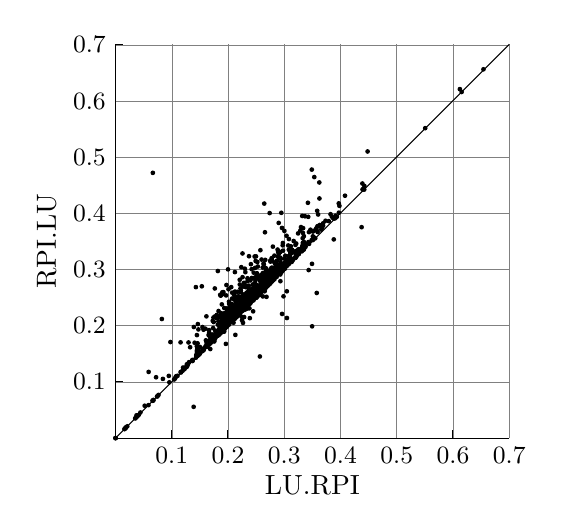
\begin{tikzpicture}

\draw (0,0) -- (5,0);
\node at (2.5,-0.6) {LU.RPI};
\node [anchor=north] at (0.714285714285714,0) {\small 0.1};
\draw (0.714285714285714,0) -- (0.714285714285714,0.1);
\draw [style=help lines] (0.714285714285714,0) -- (0.714285714285714,5);
\node [anchor=north] at (1.42857142857143,0) {\small 0.2};
\draw (1.42857142857143,0) -- (1.42857142857143,0.1);
\draw [style=help lines] (1.42857142857143,0) -- (1.42857142857143,5);
\node [anchor=north] at (2.14285714285714,0) {\small 0.3};
\draw (2.14285714285714,0) -- (2.14285714285714,0.1);
\draw [style=help lines] (2.14285714285714,0) -- (2.14285714285714,5);
\node [anchor=north] at (2.85714285714286,0) {\small 0.4};
\draw (2.85714285714286,0) -- (2.85714285714286,0.1);
\draw [style=help lines] (2.85714285714286,0) -- (2.85714285714286,5);
\node [anchor=north] at (3.57142857142857,0) {\small 0.5};
\draw (3.57142857142857,0) -- (3.57142857142857,0.1);
\draw [style=help lines] (3.57142857142857,0) -- (3.57142857142857,5);
\node [anchor=north] at (4.28571428571429,0) {\small 0.6};
\draw (4.28571428571429,0) -- (4.28571428571429,0.1);
\draw [style=help lines] (4.28571428571429,0) -- (4.28571428571429,5);
\node [anchor=north] at (5,0) {\small 0.7};
\draw (5,0) -- (5,0.1);
\draw [style=help lines] (5,0) -- (5,5);
\draw (0,0) -- (0,5);
\node [rotate=90] at (-2.5em,2.5) {RPI.LU};
\node [anchor=east] at (0,0.713285714285714) {\small 0.1};
\draw (0,0.713285714285714) -- (0.1,0.713285714285714);
\draw [style=help lines] (0,0.713285714285714) -- (5,0.713285714285714);
\node [anchor=east] at (0,1.42657142857143) {\small 0.2};
\draw (0,1.42657142857143) -- (0.1,1.42657142857143);
\draw [style=help lines] (0,1.42657142857143) -- (5,1.42657142857143);
\node [anchor=east] at (0,2.13985714285714) {\small 0.3};
\draw (0,2.13985714285714) -- (0.1,2.13985714285714);
\draw [style=help lines] (0,2.13985714285714) -- (5,2.13985714285714);
\node [anchor=east] at (0,2.85314285714286) {\small 0.4};
\draw (0,2.85314285714286) -- (0.1,2.85314285714286);
\draw [style=help lines] (0,2.85314285714286) -- (5,2.85314285714286);
\node [anchor=east] at (0,3.56642857142857) {\small 0.5};
\draw (0,3.56642857142857) -- (0.1,3.56642857142857);
\draw [style=help lines] (0,3.56642857142857) -- (5,3.56642857142857);
\node [anchor=east] at (0,4.27971428571429) {\small 0.6};
\draw (0,4.27971428571429) -- (0.1,4.27971428571429);
\draw [style=help lines] (0,4.27971428571429) -- (5,4.27971428571429);
\node [anchor=east] at (0,4.993) {\small 0.7};
\draw (0,4.993) -- (0.1,4.993);
\draw [style=help lines] (0,4.993) -- (5,4.993);

\foreach \pos in {
	(1.556186, 1.556186),
	(2.287890, 2.342277),
	(2.034038, 2.062508),
	(1.070455, 1.158038),
	(1.190476, 1.201201),
	(0.480619, 0.484526),
	(1.349544, 1.513678),
	(0.250054, 0.250054),
	(1.972249, 2.046426),
	(1.440906, 1.732451),
	(1.363287, 1.420891),
	(1.745928, 1.802097),
	(1.032574, 1.165638),
	(2.179622, 2.242647),
	(1.552430, 1.604737),
	(0.898964, 0.908736),
	(1.510241, 1.756547),
	(1.728723, 2.026342),
	(1.602943, 1.684679),
	(2.587883, 3.246073),
	(2.077456, 2.115927),
	(1.750266, 1.900922),
	(1.620730, 1.926436),
	(1.996380, 2.245221),
	(1.712040, 2.002058),
	(1.686183, 1.861827),
	(1.246753, 1.474026),
	(2.119953, 2.173218),
	(1.521739, 1.310559),
	(1.839907, 1.903352),
	(1.668702, 1.729752),
	(1.642036, 2.151067),
	(1.760131, 1.794242),
	(0.994575, 1.410488),
	(1.714286, 1.755952),
	(2.059437, 2.075078),
	(1.361273, 1.827776),
	(1.560806, 1.560806),
	(1.321892, 1.321892),
	(1.634847, 1.634847),
	(1.104901, 1.104901),
	(1.719177, 2.208315),
	(1.754729, 2.100457),
	(1.396348, 1.450054),
	(1.004318, 1.210813),
	(1.517165, 1.860465),
	(2.024264, 2.167394),
	(1.326885, 1.444692),
	(1.729911, 2.032844),
	(1.400308, 1.464543),
	(1.448652, 1.627940),
	(1.495197, 1.634645),
	(1.783416, 2.307409),
	(1.308216, 1.613466),
	(1.342857, 1.585714),
	(1.631117, 1.971680),
	(1.489621, 1.636142),
	(0.129359, 0.134983),
	(0.469764, 0.474354),
	(1.801242, 2.236025),
	(1.866475, 1.920316),
	(1.403908, 1.811800),
	(1.522052, 1.605944),
	(1.630435, 1.727484),
	(1.250955, 1.250955),
	(1.785714, 1.800115),
	(1.618804, 1.463325),
	(0.933442, 0.963880),
	(1.243622, 1.530612),
	(1.538951, 1.560178),
	(1.838755, 1.867044),
	(1.957224, 1.997579),
	(1.535598, 1.713975),
	(1.710076, 1.710076),
	(1.394286, 1.577143),
	(1.392857, 1.464286),
	(1.553288, 1.575964),
	(1.815062, 1.887304),
	(1.617681, 1.822739),
	(1.251476, 1.227863),
	(1.194162, 1.194162),
	(1.661753, 1.755562),
	(1.813616, 1.813616),
	(1.624030, 1.925841),
	(2.376477, 2.537594),
	(1.551459, 1.628264),
	(1.720210, 1.742994),
	(1.655052, 1.916376),
	(1.941610, 2.097506),
	(1.562500, 1.596841),
	(0.267681, 0.267681),
	(1.926164, 1.926164),
	(0.267857, 0.287698),
	(0.267857, 0.287698),
	(1.251618, 1.273198),
	(1.071429, 1.071429),
	(1.020408, 1.916980),
	(0.850181, 0.853528),
	(0.676692, 0.789474),
	(0.875576, 0.875576),
	(0.115830, 0.115830),
	(1.392857, 1.392857),
	(1.344086, 1.344086),
	(1.344086, 1.344086),
	(0.418443, 0.418443),
	(1.561022, 1.655629),
	(0.315770, 0.324863),
	(0.127767, 0.127767),
	(0.127767, 0.129112),
	(0.545889, 0.548326),
	(0.369922, 0.410277),
	(1.034964, 1.099314),
	(0.294922, 0.294922),
	(1.059771, 1.066836),
	(1.378245, 1.355370),
	(0.473934, 3.368314),
	(0.527024, 0.527024),
	(0.683230, 0.708075),
	(1.104323, 1.409774),
	(1.235231, 1.235231),
	(0.253593, 0.253593),
	(1.751152, 1.751152),
	(1.095994, 1.927438),
	(0.992063, 0.396825),
	(0.601504, 0.751880),
	(0.480769, 0.480769),
	(0.514801, 0.772201),
	(1.749271, 1.749271),
	(0.588235, 1.512605),
	(1.632653, 1.632653),
	(0.000000, 0.000000),
	(0.148810, 0.148810),
	(1.020408, 1.020408),
	(0.696864, 1.219512),
	(0.744048, 0.744048),
	(0.533049, 0.533049),
	(1.166181, 1.166181),
	(1.288056, 1.522248),
	(0.420168, 0.840336),
	(0.000000, 0.000000),
	(1.428571, 2.142857),
	(3.125000, 2.678571),
	(4.395604, 4.395604),
	(1.586670, 1.899454),
	(2.175244, 1.864130),
	(1.744072, 1.949833),
	(1.187591, 1.371096),
	(1.531900, 1.728143),
	(1.572865, 1.692539),
	(2.033262, 2.120792),
	(1.142061, 1.388778),
	(1.338802, 1.547748),
	(1.843231, 1.940670),
	(1.676689, 1.836503),
	(1.694212, 1.792318),
	(1.365061, 1.542395),
	(1.412464, 1.455830),
	(1.198943, 1.283614),
	(2.406748, 2.816901),
	(1.285925, 1.563488),
	(1.802911, 2.038230),
	(1.820728, 1.884921),
	(1.651348, 1.701979),
	(1.515290, 1.538110),
	(1.600731, 1.709805),
	(2.004808, 2.051342),
	(1.034028, 1.078029),
	(1.837379, 1.837379),
	(1.882698, 2.205523),
	(2.475999, 2.646262),
	(1.381034, 1.651504),
	(2.128173, 2.134208),
	(1.537839, 1.537839),
	(1.987146, 2.164359),
	(2.105427, 2.105427),
	(1.496313, 1.607786),
	(1.839767, 2.386194),
	(1.464179, 1.597045),
	(1.369963, 1.853480),
	(1.587302, 1.591711),
	(2.073922, 2.340862),
	(1.983941, 2.134493),
	(2.447045, 2.809749),
	(1.678257, 1.713848),
	(1.998149, 2.082282),
	(1.675048, 1.791912),
	(1.698166, 1.806559),
	(1.962624, 2.099460),
	(1.515869, 2.108006),
	(2.403414, 2.425876),
	(1.434531, 1.890005),
	(1.657754, 1.791444),
	(1.776185, 1.802866),
	(1.966279, 1.985603),
	(1.306973, 1.480685),
	(1.954115, 1.984127),
	(1.344390, 1.470034),
	(2.321249, 2.335578),
	(1.254181, 1.230291),
	(2.496633, 1.419248),
	(1.817867, 1.936585),
	(2.262094, 2.502839),
	(1.531737, 1.539613),
	(1.336779, 1.813564),
	(1.675898, 2.029221),
	(1.692737, 1.936119),
	(1.324194, 1.417666),
	(1.982212, 2.261445),
	(2.040241, 2.140845),
	(1.766600, 2.305835),
	(1.443093, 1.443093),
	(1.378106, 1.378106),
	(1.453373, 1.661706),
	(2.125066, 2.477596),
	(1.979658, 1.988277),
	(1.890915, 1.901705),
	(0.113773, 0.114527),
	(1.503759, 1.597744),
	(1.051709, 1.139351),
	(1.331558, 1.464714),
	(1.735834, 1.900439),
	(1.394155, 1.493321),
	(1.761834, 1.793674),
	(1.387363, 1.575092),
	(2.060762, 2.306489),
	(1.640146, 1.675705),
	(1.797424, 1.812061),
	(1.141527, 1.163693),
	(2.555408, 1.842842),
	(1.376804, 1.508977),
	(1.220488, 1.293851),
	(2.119514, 2.131964),
	(1.355534, 1.850706),
	(2.098404, 2.275112),
	(1.591441, 1.873536),
	(1.325848, 1.391543),
	(2.142560, 2.175203),
	(1.675557, 1.808905),
	(1.501966, 1.627785),
	(1.764079, 1.810678),
	(2.097527, 2.228958),
	(1.968380, 2.037667),
	(1.300044, 1.440390),
	(2.382885, 2.481447),
	(1.808395, 1.814443),
	(1.498423, 1.464624),
	(1.566475, 1.566475),
	(1.361139, 1.467283),
	(1.575290, 1.575290),
	(1.503759, 1.564395),
	(1.487100, 1.684185),
	(1.749971, 1.772847),
	(2.077654, 2.188168),
	(1.442929, 1.514716),
	(1.594286, 1.634286),
	(1.604295, 1.539212),
	(1.675406, 1.710577),
	(2.318548, 2.599366),
	(1.401230, 1.196172),
	(1.791675, 1.784863),
	(1.217965, 1.243339),
	(2.038509, 2.161272),
	(1.897547, 1.897547),
	(0.825688, 1.215596),
	(1.504414, 1.647395),
	(1.037102, 1.080923),
	(1.362835, 1.507135),
	(1.657716, 1.672037),
	(2.333044, 2.356441),
	(1.515152, 1.515152),
	(2.114967, 1.576542),
	(1.782247, 1.782247),
	(1.319261, 1.319261),
	(2.327554, 2.336977),
	(1.888574, 2.977877),
	(2.023875, 2.221519),
	(2.492651, 3.409759),
	(2.294343, 2.470830),
	(2.592257, 2.705456),
	(1.762918, 1.863602),
	(2.055279, 2.076169),
	(1.451696, 1.622987),
	(1.189882, 1.339508),
	(2.147440, 2.223823),
	(1.845883, 1.881462),
	(1.967478, 2.241101),
	(1.729115, 2.145121),
	(1.612379, 2.344689),
	(1.632377, 1.728967),
	(1.420904, 1.440073),
	(1.578216, 1.950282),
	(1.495215, 1.677489),
	(1.869398, 2.165722),
	(1.772814, 1.818885),
	(1.454784, 1.643512),
	(1.788087, 1.808967),
	(2.412670, 2.429586),
	(1.472370, 1.480135),
	(1.466783, 1.488676),
	(2.495288, 2.212590),
	(1.894320, 1.917962),
	(1.689890, 1.713996),
	(1.626184, 1.821737),
	(1.783634, 1.864078),
	(2.031056, 2.105590),
	(1.663276, 1.845992),
	(1.762005, 1.791954),
	(2.076180, 2.164018),
	(2.183990, 2.209045),
	(1.851003, 1.887657),
	(2.065121, 2.363503),
	(2.375992, 2.415675),
	(1.808556, 1.932172),
	(2.382475, 2.665723),
	(1.611868, 1.676057),
	(2.135383, 2.188768),
	(1.633177, 1.536838),
	(1.887631, 1.957185),
	(1.629223, 1.660664),
	(1.117300, 1.376147),
	(1.710821, 1.712625),
	(1.226593, 1.238858),
	(1.700334, 1.759919),
	(2.072264, 2.732655),
	(1.839259, 1.858000),
	(1.789455, 1.852295),
	(1.378043, 1.351542),
	(1.756292, 1.946406),
	(2.057873, 2.196001),
	(2.836015, 2.862425),
	(1.572823, 1.606158),
	(1.489970, 1.491578),
	(2.032367, 2.131835),
	(1.847635, 1.905561),
	(2.011952, 2.046101),
	(1.591822, 1.622336),
	(1.531188, 1.670875),
	(1.384083, 1.586752),
	(1.765717, 1.833707),
	(1.519914, 1.684428),
	(1.718278, 1.872033),
	(1.893842, 1.865691),
	(2.379232, 2.477291),
	(1.808954, 1.874278),
	(1.875119, 1.881448),
	(2.374535, 2.445129),
	(1.893018, 2.079095),
	(1.862976, 2.028380),
	(1.153822, 1.545866),
	(1.203071, 1.130524),
	(2.146034, 2.212466),
	(1.383163, 1.532533),
	(1.254010, 1.254010),
	(2.077160, 2.289628),
	(2.205987, 2.310611),
	(1.442211, 1.470293),
	(1.397789, 1.451187),
	(1.668802, 1.832159),
	(1.499353, 1.624933),
	(1.626941, 1.717108),
	(2.449194, 2.489140),
	(1.383526, 1.544402),
	(1.391891, 1.535993),
	(1.646168, 1.632923),
	(1.880081, 2.217625),
	(1.771255, 1.818248),
	(1.052265, 1.379791),
	(1.341132, 1.559731),
	(1.654280, 1.929535),
	(1.611082, 1.625194),
	(1.474886, 1.499697),
	(2.043613, 2.098422),
	(2.159548, 2.179985),
	(1.849571, 1.897464),
	(1.539288, 1.793890),
	(1.238938, 1.396966),
	(1.323676, 1.402764),
	(1.505266, 1.817193),
	(1.795777, 1.866989),
	(1.045770, 1.059639),
	(1.630812, 1.670467),
	(1.537232, 1.550016),
	(1.580370, 1.701670),
	(1.794193, 1.872202),
	(1.705473, 1.523229),
	(1.469150, 1.522930),
	(1.353591, 1.515391),
	(1.579652, 1.661519),
	(1.427123, 1.470588),
	(1.531051, 1.564801),
	(1.729160, 1.803533),
	(2.365037, 2.371403),
	(1.422329, 1.582843),
	(1.893524, 1.897444),
	(1.809618, 1.905234),
	(2.219283, 2.333186),
	(2.200772, 2.209965),
	(2.506510, 2.622768),
	(2.193017, 2.445758),
	(1.802089, 1.887060),
	(2.171492, 2.569201),
	(1.412873, 1.439037),
	(2.511808, 2.527142),
	(1.045296, 1.447333),
	(2.203826, 2.304508),
	(1.647555, 1.941144),
	(1.700159, 1.648141),
	(1.456767, 1.625157),
	(2.092555, 2.363271),
	(1.682253, 1.709126),
	(1.786857, 1.896536),
	(1.785094, 1.947713),
	(1.036933, 1.127820),
	(2.099666, 2.113921),
	(2.311745, 2.351874),
	(1.826880, 1.873678),
	(1.637749, 1.790174),
	(1.400232, 1.493174),
	(2.098353, 2.162884),
	(1.669440, 1.712924),
	(1.828328, 1.816153),
	(1.768833, 2.037065),
	(1.747482, 1.609474),
	(1.560796, 1.665304),
	(1.840812, 1.858253),
	(1.751492, 1.797122),
	(1.807419, 2.178374),
	(1.856951, 1.962605),
	(1.627968, 1.762656),
	(2.299766, 2.309133),
	(1.541943, 1.590930),
	(1.628007, 1.711998),
	(2.560922, 2.885598),
	(2.243590, 2.389674),
	(1.767968, 1.867791),
	(1.645574, 1.696880),
	(1.452330, 1.486818),
	(1.192591, 1.236996),
	(1.266373, 1.270211),
	(1.923408, 1.942054),
	(1.577164, 2.009906),
	(1.302232, 1.527108),
	(2.507015, 2.515148),
	(1.898485, 1.966366),
	(2.132984, 1.800064),
	(2.036762, 2.189574),
	(2.285101, 2.453800),
	(2.113763, 2.668923),
	(1.964602, 2.252845),
	(1.738473, 1.747366),
	(1.897526, 1.933306),
	(1.702393, 1.721575),
	(1.736094, 1.824308),
	(1.364210, 1.504327),
	(1.234538, 1.489207),
	(2.087097, 2.087097),
	(1.698806, 1.744720),
	(1.977848, 2.158680),
	(1.814809, 1.848541),
	(1.899673, 1.948437),
	(1.693841, 1.702289),
	(1.998251, 2.431524),
	(1.943060, 2.012757),
	(1.070006, 1.092772),
	(1.355271, 1.537204),
	(2.621746, 2.669490),
	(1.995565, 2.038328),
	(1.469311, 1.916784),
	(1.627434, 1.656275),
	(1.391290, 1.431813),
	(1.898734, 2.022303),
	(2.286076, 2.304147),
	(1.791097, 1.877227),
	(2.086301, 2.086301),
	(1.625631, 1.705403),
	(1.431413, 1.584144),
	(1.613008, 2.043359),
	(1.836461, 1.920720),
	(1.299369, 2.121568),
	(1.546518, 1.580776),
	(1.259863, 1.296918),
	(1.832942, 1.036455),
	(1.438383, 1.517222),
	(1.677041, 1.839086),
	(1.930023, 2.069906),
	(1.987215, 2.016994),
	(2.062723, 2.193807),
	(1.832516, 1.840426),
	(2.083051, 2.141729),
	(1.572899, 1.692849),
	(2.519119, 2.549709),
	(1.335205, 1.808566),
	(2.249473, 2.265094),
	(1.826061, 1.876868),
	(1.796442, 2.092923),
	(1.719945, 1.830481),
	(1.775939, 1.802692),
	(1.546425, 1.634327),
	(1.414824, 1.646809),
	(1.887039, 1.965484),
	(2.387984, 2.463927),
	(1.482290, 1.505792),
	(1.394069, 1.538605),
	(1.801298, 1.846438),
	(1.984347, 2.120515),
	(2.048752, 2.192524),
	(1.589338, 1.853791),
	(1.610707, 1.727733),
	(1.632170, 1.684760),
	(1.549480, 1.857197),
	(1.957408, 2.050429),
	(1.858006, 1.879586),
	(1.430515, 1.593780),
	(1.340111, 1.350013),
	(1.641545, 1.690364),
	(1.263142, 1.270616),
	(1.612848, 1.647164),
	(1.909477, 1.942480),
	(2.635892, 2.697350),
	(1.602488, 1.620315),
	(1.412663, 1.568565),
	(2.073593, 2.145743),
	(1.517067, 1.580278),
	(1.863580, 1.889535),
	(1.510949, 1.533717),
	(1.973684, 2.030430),
	(2.073234, 2.088706),
	(2.236386, 2.236386),
	(1.619337, 1.643182),
	(1.801837, 1.899551),
	(1.288265, 1.353635),
	(2.105394, 2.860858),
	(1.682300, 1.817758),
	(1.053384, 1.054300),
	(1.510470, 1.851307),
	(1.288154, 1.306003),
	(1.546919, 1.655820),
	(2.843310, 2.948944),
	(1.884841, 2.031376),
	(2.009978, 2.067543),
	(1.478823, 1.574539),
	(2.304933, 2.380525),
	(1.614907, 1.784897),
	(1.464765, 1.541409),
	(1.483227, 1.560458),
	(1.645591, 1.714617),
	(1.566166, 1.602625),
	(1.917649, 2.051117),
	(1.602816, 1.638216),
	(2.142751, 2.174653),
	(1.941406, 1.952237),
	(1.871650, 1.880735),
	(1.917606, 1.793473),
	(1.750732, 1.856492),
	(2.246004, 2.355136),
	(2.322498, 2.398061),
	(1.775784, 1.915977),
	(1.504827, 1.636651),
	(1.594460, 1.716863),
	(1.555071, 1.648855),
	(1.481285, 1.847009),
	(3.137066, 3.156938),
	(1.358589, 1.503245),
	(2.208992, 2.312902),
	(1.868323, 1.869565),
	(1.514856, 1.559755),
	(1.609885, 1.684088),
	(1.913709, 2.044604),
	(2.226589, 2.435065),
	(1.711722, 1.755080),
	(1.835585, 2.051832),
	(1.326324, 1.367319),
	(1.484980, 1.571632),
	(2.045954, 2.047952),
	(1.886705, 1.993499),
	(1.417445, 1.494848),
	(2.052899, 2.095187),
	(1.700106, 1.719716),
	(2.000471, 2.009885),
	(1.931649, 1.972334),
	(2.221111, 2.358564),
	(1.272718, 1.341118),
	(2.388601, 2.415721),
	(1.442239, 1.460222),
	(1.817961, 1.878661),
	(1.421137, 1.478132),
	(1.225555, 1.281505),
	(1.902421, 1.898290),
	(2.156244, 2.226366),
	(1.588889, 1.787500),
	(1.743085, 1.764136),
	(1.563544, 1.618669),
	(1.914553, 2.132176),
	(2.378319, 2.413085),
	(1.389245, 1.427717),
	(0.946980, 1.153696),
	(2.223814, 2.352079),
	(2.126636, 2.135549),
	(1.511381, 1.767048),
	(1.310380, 1.376756),
	(2.211860, 2.251245),
	(2.122959, 2.447279),
	(1.670795, 1.703826),
	(2.443057, 2.988029),
	(1.476190, 1.680556),
	(2.012490, 2.053514),
	(1.937736, 1.944159),
	(1.624234, 1.685526),
	(1.902349, 1.918436),
	(1.441603, 1.504724),
	(1.651948, 1.688312),
	(1.448953, 1.532333),
	(1.849003, 1.887458),
	(1.614231, 1.673678),
	(3.158141, 3.155542),
	(1.985400, 2.013225),
	(2.536341, 2.537594),
	(2.523984, 3.314720),
	(1.487741, 1.555688),
	(1.638916, 1.766122),
	(1.791375, 1.894530),
	(1.533923, 1.620312),
	(2.242884, 2.276268),
	(1.532980, 1.740139),
	(1.870102, 2.095135),
	(1.328904, 1.819516),
	(1.418847, 1.617751),
	(1.912342, 1.933016),
	(1.511370, 1.543063),
	(2.566674, 2.616819),
	(1.848164, 1.893735),
	(1.448312, 1.651761),
	(1.754951, 1.772530),
	(1.785714, 1.785714),
	(2.211038, 2.292769),
	(1.917073, 1.950051),
	(1.912613, 1.919381),
	(2.218768, 2.271259),
	(1.783962, 1.845297),
	(1.291069, 1.334180),
	(1.573098, 1.643535),
	(1.748905, 1.791999),
	(1.519003, 1.581514),
	(1.414709, 1.556890),
	(1.769512, 1.967870),
	(1.730722, 1.771966),
	(2.222737, 2.242031),
	(2.094718, 2.130858),
	(1.748478, 1.778082),
	(2.393368, 2.400053),
	(1.845539, 1.985402),
	(1.897679, 1.925922),
	(2.050594, 2.131358),
	(1.601597, 1.739130),
	(2.371576, 2.427833),
	(1.408304, 1.943564),
	(1.945764, 2.016897),
	(1.958933, 1.957603),
	(1.484368, 1.580203),
	(1.694675, 2.309487),
	(2.108148, 2.183714),
	(2.746722, 2.812284),
	(1.829441, 2.001198),
	(2.730487, 2.843097),
	(1.990447, 2.096017),
	(1.462054, 1.495536),
	(1.276596, 1.297558),
	(2.287893, 2.291298),
	(1.789421, 1.799798),
	(1.342433, 1.429266),
	(1.513538, 1.556139),
	(2.045410, 2.098538),
	(1.532143, 1.673214),
	(1.566048, 1.596900),
	(1.700316, 1.707956),
	(1.681095, 1.727113),
	(1.554635, 1.623680),
	(1.913406, 2.024726),
	(1.698084, 1.701979),
	(1.456541, 1.540978),
	(1.942895, 2.097318),
	(2.001840, 2.069246),
	(2.180196, 2.197535),
	(2.169258, 2.242256),
	(1.596237, 1.685188),
	(2.093787, 1.992326),
	(2.093833, 2.290846),
	(1.903236, 2.109229),
	(1.762077, 1.792775),
	(2.535368, 2.640777),
	(2.037206, 2.113032),
	(1.261012, 1.900155),
	(2.041033, 2.063796),
	(1.722429, 1.806450),
	(1.845939, 1.888702),
	(2.196621, 2.230756),
	(1.593880, 1.783102),
	(2.156024, 2.315120),
	(1.587302, 1.701528),
	(1.970894, 2.018823),
	(1.978670, 2.054098),
	(1.624225, 1.680233),
	(1.896240, 1.923212),
	(2.007136, 2.086148),
	(1.644238, 1.667869),
	(1.568570, 1.625376),
	(1.674945, 1.645312),
	(2.064494, 2.154679),
	(1.541637, 1.679828),
	(2.516153, 2.543193),
	(2.060639, 2.099988),
	(1.181365, 1.308916),
	(1.852363, 1.906371),
	(1.724199, 1.789229),
	(1.776190, 2.007410),
	(1.567874, 1.749949),
	(1.597106, 2.170652),
	(2.144300, 2.630592),
	(1.727490, 1.810523),
	(1.717991, 1.822853),
	(1.779086, 2.248383),
	(1.963587, 2.021065),
	(1.719331, 1.776863),
	(1.539936, 1.549656),
	(1.429029, 1.445034),
	(1.933861, 1.976297),
	(1.791537, 2.067158),
	(2.200963, 2.391713),
	(1.720409, 1.745688),
	(1.302496, 1.352592),
	(2.149709, 2.225363),
	(2.403138, 2.449870),
	(1.561605, 1.801683),
	(1.575414, 1.578561),
	(1.843799, 1.848769),
	(2.343906, 2.400100),
	(1.943103, 1.974778),
	(1.410962, 1.522413),
	(2.011352, 2.074933),
	(2.017722, 2.317088),
	(1.349903, 1.697507),
	(2.015327, 2.072365),
	(2.314453, 2.371067),
	(1.594474, 1.726809),
	(1.781893, 1.923833),
	(1.854314, 2.267327),
	(1.791626, 1.797190),
	(1.616367, 1.622793),
	(2.227188, 2.276200),
	(1.902490, 2.161100),
	(1.457396, 1.538281),
	(1.940402, 1.975052),
	(1.519791, 1.536081),
	(1.587667, 1.636425),
	(1.207614, 1.208387),
	(3.201123, 3.639874),
	(1.543350, 1.550483),
	(0.473271, 0.474155),
	(1.760097, 1.873022),
	(1.647522, 1.666088),
	(1.530171, 1.549277),
	(1.416229, 1.416229),
	(0.754647, 0.755194),
	(1.307947, 1.308831),
	(2.563598, 2.689109),
	(1.982926, 2.284598),
	(1.649334, 1.687628),
	(1.493414, 1.579833),
	(1.913486, 2.152980),
	(1.507043, 1.510873),
	(1.910425, 1.932046),
	(1.771486, 1.808629),
	(1.232687, 1.255111),
	(1.704853, 1.712349),
	(1.786143, 1.861663),
	(1.656956, 1.707801),
	(1.356705, 1.364668),
	(1.339286, 1.365248),
	(1.990393, 2.027209),
	(1.408920, 1.413438),
	(1.339947, 1.372354),
	(1.060665, 1.062902),
	(2.131391, 2.156643),
	(1.659589, 1.665612),
	(2.032351, 2.077194),
	(2.794407, 2.825160),
	(1.033744, 1.307738),
	(1.235944, 1.287174),
	(2.635914, 2.727112),
	(2.220332, 2.262869),
	(1.921268, 1.974911),
	(2.452853, 2.133613),
	(1.156451, 1.160151),
	(2.149875, 2.149875),
	(2.811018, 2.811018),
	(1.956766, 2.128644),
	(1.871162, 1.798749),
	(1.849905, 1.914527),
	(1.897690, 2.613744),
	(1.442733, 1.703841),
	(1.840725, 1.861825),
	(1.956908, 2.857525),
	(1.515348, 1.527374),
	(2.071268, 2.187902),
	(1.541468, 1.587991),
	(2.370698, 2.820611),
	(1.933800, 1.945374),
	(1.896654, 1.963491),
	(1.513891, 1.524586),
	(1.783617, 1.854338),
	(1.849737, 1.927602),
	(1.881852, 1.970945),
	(1.261186, 1.544026),
	(1.693828, 1.890894),
	(1.854093, 2.002953),
	(1.795388, 1.797967),
	(1.831472, 1.880663),
	(1.479904, 1.771516),
	(1.829553, 1.845141),
	(2.306199, 2.335310),
	(1.570205, 1.572059),
	(2.017395, 2.016006),
	(2.114387, 2.132102),
	(1.548001, 1.608863),
	(2.145476, 2.163423),
	(1.777246, 1.791297),
	(1.980084, 1.985829),
	(1.641643, 1.788124),
	(1.153357, 1.225095),
	(1.940642, 1.940907),
	(2.547906, 2.661356),
	(2.247022, 2.258527),
	(1.788491, 1.905669),
	(1.652420, 1.658077),
	(1.772939, 2.161942),
	(1.060540, 1.077195),
	(1.272011, 1.325243),
	(1.817597, 1.895109),
	(1.162976, 1.182797),
	(1.303850, 1.308206),
	(1.402132, 1.462897),
	(1.772444, 1.777269),
	(1.299856, 1.316872),
	(1.154559, 1.176763),
	(1.515685, 1.633466),
	(2.176489, 1.524880),
	(2.346517, 2.376033),
	(1.616848, 1.791758),
	(2.355282, 2.679374),
	(1.228278, 1.238410),
	(1.331963, 1.359541),
	(2.707968, 2.755216),
	(1.504362, 1.524401),
	(2.572688, 2.839572),
	(2.304355, 2.336539),
	(1.253043, 1.301596),
	(1.051973, 1.058548),
	(1.574651, 1.581604),
	(1.377014, 1.391316),
	(3.134557, 3.232853),
	(1.171827, 1.193389),
	(1.429962, 1.446871),
	(1.036725, 1.051891),
	(2.090560, 2.210339),
	(1.575183, 1.626349),
	(0.280112, 0.280112),
	(1.340367, 1.369925),
	(1.562908, 1.575139),
	(2.092219, 2.078069),
	(1.648816, 2.107155),
	(1.772586, 1.894260),
	(2.182940, 2.238143),
	(2.058135, 2.393958),
	(1.890587, 1.867601),
	(1.989763, 1.992069),
	(1.798711, 1.802870),
	(2.101905, 2.106430),
	(1.696480, 1.812243),
	(2.283578, 2.371529),
	(2.134378, 2.179697),
	(1.879130, 1.967142),
	(1.832168, 1.876348),
	(1.623926, 1.711939),
	(1.901861, 2.263083),
	(2.031832, 2.102724),
	(1.849870, 2.071222),
	(1.392554, 1.547514),
	(1.998750, 2.044422),
	(1.893699, 1.969349),
	(2.050183, 2.252188),
	(2.206681, 2.284764),
	(2.393489, 2.489517),
	(1.480314, 1.503657),
	(1.717090, 1.730161),
	(2.346541, 2.635364),
	(1.983615, 2.124936),
	(1.849063, 1.969784),
	(1.909869, 1.924919),
	(1.213367, 1.229835),
	(2.505967, 2.561979),
	(2.118378, 2.122305),
	(2.313152, 2.352855),
	(2.763797, 2.793730),
	(1.965494, 1.965967),
	(1.878462, 2.011704),
	(1.227904, 1.315237),
	(2.201716, 2.527642),
	(1.466313, 1.495667),
	(1.630454, 1.674587),
	(1.325795, 1.342955),
	(1.372929, 1.439132),
	(1.521653, 1.523548),
	(1.567786, 1.654166),
	(0.911701, 0.916913),
	(1.545672, 1.668971),
	(1.178899, 1.209515),
	(1.384740, 1.390191),
	(2.085506, 2.193040),
	(1.514841, 1.536779),
	(1.409673, 1.424210),
	(1.991162, 2.009253),
	(2.368085, 2.385389),
	(1.039881, 1.041705),
	(1.606614, 1.494771),
	(2.290779, 2.300907),
	(2.835160, 2.980770),
	(0.926814, 1.214446),
	(2.062145, 2.157710),
	(1.673108, 1.682132),
	(1.736780, 1.787293),
	(2.797087, 2.799451),
	(0.906042, 0.937365),
	(2.043012, 2.093888),
	(2.174230, 2.183958),
	(1.329249, 1.367908),
	(1.560969, 1.596560),
	(1.937046, 1.957596),
	(1.853702, 1.862027),
	(2.772275, 2.789159),
	(2.203896, 2.313731),
	(0.902256, 0.902256),
	(1.724138, 1.736453),
	(1.265408, 1.364948),
	(1.450768, 1.556410),
	(1.547633, 1.562474),
	(1.501233, 1.510074),
	(1.962608, 1.979731),
	(2.138215, 2.183313),
	(2.456187, 2.615507),
	(1.372267, 1.421625),
	(2.397984, 2.444485),
	(1.687873, 1.717086),
	(1.774753, 1.785043),
	(1.343794, 1.342380),
	(1.213325, 1.226423),
	(1.493343, 1.505712),
	(3.932592, 3.935914),
	(1.878264, 1.886057),
	(2.006544, 2.020036),
	(2.379380, 2.605763),
	(2.490602, 2.514098),
	(1.676300, 1.993174),
	(1.758741, 1.783338),
	(1.147471, 1.241576),
	(1.436561, 1.455996),
	(2.159021, 2.266780),
	(0.867188, 0.873373),
	(1.213495, 1.235051),
	(2.406319, 2.465414),
	(2.110107, 2.128992),
	(2.555130, 2.637773),
	(2.310924, 2.335363),
	(1.183844, 1.186956),
	(1.380617, 1.442494),
	(1.467927, 1.510831),
	(1.304580, 1.312175),
	(1.697260, 1.709505),
	(1.291531, 1.299640),
	(0.976240, 0.992400),
	(3.159460, 3.202825),
	(1.902555, 1.950448),
	(2.387880, 2.390703),
	(2.247805, 2.255786),
	(1.116554, 1.119892),
	(2.572406, 2.691556),
	(1.610759, 1.614669),
	(1.362183, 1.365348),
	(1.597926, 1.610770),
	(1.575701, 1.674147),
	(1.478795, 1.702009),
	(1.460925, 1.476341),
	(2.391881, 2.564403),
	(1.361958, 1.378588),
	(1.120691, 1.121476),
	(1.467319, 1.489097),
	(4.672151, 4.683293),
	(1.528951, 1.566165),
	(1.554970, 1.555348),
	(1.894891, 1.908819),
	(2.311082, 2.378093),
	(1.157387, 1.192900),
	(1.479758, 1.494070),
	(1.175961, 1.188644),
	(1.339698, 1.371453),
	(2.457955, 2.466654),
	(1.236044, 1.244483),
	(2.000414, 2.004557),
	(1.373242, 1.376854),
	(0.760425, 0.769216),
	(1.036132, 1.061715),
	(1.341753, 1.348672),
	(1.390107, 1.428627),
	(0.769962, 0.785401),
	(1.208047, 1.212964),
	(1.257759, 1.273444),
	(0.830060, 0.832470),
	(1.299411, 1.302211),
	(1.110715, 1.134739),
	(1.780798, 1.786417),
	(3.143389, 3.161387),
	(1.089676, 1.099353),
	(1.451773, 1.470415),
	(1.375346, 1.377475),
	(1.254443, 1.277873),
	(1.633536, 1.650159),
	(0.977969, 0.979379),
	(1.153417, 1.159999),
	(0.971210, 0.982292),
	(1.213915, 1.243570),
	(2.612147, 2.648283),
	(2.784731, 2.789201),
	(0.919622, 0.937811),
	(1.261426, 1.263335),
	(1.224602, 1.226493),
	(1.034082, 1.110657),
	(0.826802, 0.839413),
	(2.589468, 3.042867),
	(1.793877, 1.811448),
	(1.374330, 1.389331),
	(2.666914, 2.759495),
	(1.318575, 1.335390),
	(1.103767, 1.113074),
	(0.976598, 0.982039),
	(0.786973, 0.790781),
	(1.042000, 1.203548),
	(1.263201, 1.265788),
	(1.702189, 1.795092),
	(0.857639, 0.895446),
	(1.024628, 1.053475),
	(2.147729, 2.278884),
	(2.281822, 2.287931),
	(1.513813, 1.589207),
	(2.186309, 2.201968),
	(2.230842, 2.267998),
	(1.651383, 1.661558),
	(4.372778, 4.431567),
	(1.423293, 1.431956),
	(1.306790, 1.308565),
	(0.870040, 0.878465),
	(1.314863, 1.355689),
	(1.852380, 1.854164),
	(1.225205, 1.262126),
	(1.118317, 1.131213),
	(1.708601, 1.721521),
	(1.589145, 1.765181),
	(2.126998, 2.380434),
	(2.914077, 3.078018),
	(1.541670, 1.548534),
	(1.110520, 1.117626),
	(2.771855, 2.523099),
} \fill \pos circle(0.03);

\draw (0,0) -- (5, 5);

\end{tikzpicture}

\end{frame}


\section{Difficulties}
\subsection{to find a combined algorithm always at least as good as both compositions}

\begin{frame}{Irregular Units}
  \begin{center}
\begin{tikzpicture}[node distance=1.3cm]
  \proofnode[color=addcolor]{luroot}{\only<4>{$\bot$}};

  \proofnode[above left of=luroot]{root}{\alt<3-4>{$\bar{a}$}{$\bot$}};
  \withchildren{root} {r2}{\alt<3-4>{$\bar{a} c$}{$c$}} {a4}{$\bar{c}$};
  \withchildren{r2} {r0}{\alt<8>{$b c$}{$b$}} {r1}{$\bar{b} c$};

  \addchildren{r0} {a0}{$\bar{a} b$} {iu}{$a$};
  \draw [proof edge] (r0) -- (a0);
  \only<1,5->{\draw [proof edge] (r0) -- (iu);}
  \only<2>{\draw [deleted edge] (r0) -- (iu);}

  \addchildren{iu} {a1}{$a c$} {a2}{$a \bar{c}$};
  \draw [proof edge] (iu) -- (a1);
  \only<1-6>{\draw [proof edge] (iu) -- (a2);}
  \only<7>{\draw [deleted edge] (iu) -- (a2);}

  \proofnode[above right of=r1]{a3}{$\bar{a} \bar{b} c$};
  \draw [proof edge] (r1) -- (a3);
  \only<1,5->{\draw [proof edge] (r1) -- (iu);}
  \only<2>{\draw [deleted edge] (r1) -- (iu);}

  \crossnode<3-4>{r0}
  \crossnode<3-4>{r1}
  \only<4>{
    \draw [proof edge,color=addcolor] (luroot) -- (root);
    \draw [proof edge,color=addcolor] (luroot) .. controls ++(1.2,1.5) .. (iu);
  }

  \pivot<6-7>{iu}{$c$}
  \pivot<6->{root}{$c$}
  \crossnode<8>{a2}
  \crossnode<8>{iu}

  \draw (luroot) ++(1.2,-0.5) node {};
\end{tikzpicture}
\end{center}
\end{frame}

\begin{frame}{Root Safe Literals}
\end{frame}

\begin{frame}{Units introduced by RPI}
\end{frame}

\begin{frame}{Back to Irregular Units}
\end{frame}


\section{Combined Equivalents}
\subsection{to both sequential compositions}

\begin{frame}{RPI[3]LU}
\end{frame}

\begin{frame}{LUnivRPI}
\end{frame}

\section{LowerUnivalents}
\subsection{A new algorithm extending LU}

\begin{frame}{Formal Presentation}
\end{frame}

\begin{frame}{Implementation}
\end{frame}


\appendix

\begin{frame}{Conclusion}
\centering
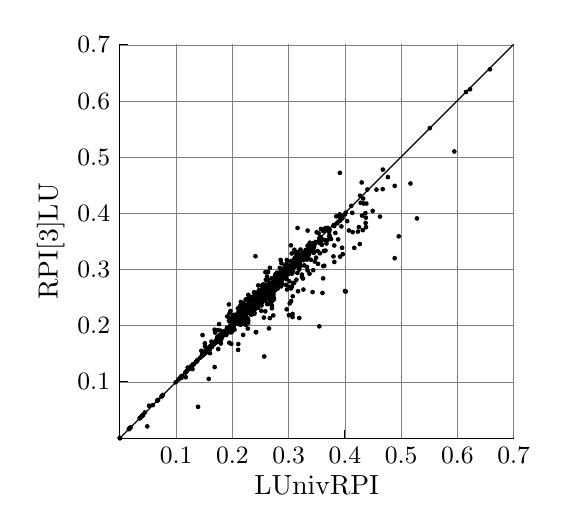
\begin{tikzpicture}

\draw (0,0) -- (5,0);
\node at (2.5,-0.6) {LUnivRPI};
\node [anchor=north] at (0.714285714285714,0) {\small 0.1};
\draw (0.714285714285714,0) -- (0.714285714285714,0.1);
\draw [style=help lines] (0.714285714285714,0) -- (0.714285714285714,5);
\node [anchor=north] at (1.42857142857143,0) {\small 0.2};
\draw (1.42857142857143,0) -- (1.42857142857143,0.1);
\draw [style=help lines] (1.42857142857143,0) -- (1.42857142857143,5);
\node [anchor=north] at (2.14285714285714,0) {\small 0.3};
\draw (2.14285714285714,0) -- (2.14285714285714,0.1);
\draw [style=help lines] (2.14285714285714,0) -- (2.14285714285714,5);
\node [anchor=north] at (2.85714285714286,0) {\small 0.4};
\draw (2.85714285714286,0) -- (2.85714285714286,0.1);
\draw [style=help lines] (2.85714285714286,0) -- (2.85714285714286,5);
\node [anchor=north] at (3.57142857142857,0) {\small 0.5};
\draw (3.57142857142857,0) -- (3.57142857142857,0.1);
\draw [style=help lines] (3.57142857142857,0) -- (3.57142857142857,5);
\node [anchor=north] at (4.28571428571429,0) {\small 0.6};
\draw (4.28571428571429,0) -- (4.28571428571429,0.1);
\draw [style=help lines] (4.28571428571429,0) -- (4.28571428571429,5);
\node [anchor=north] at (5,0) {\small 0.7};
\draw (5,0) -- (5,0.1);
\draw [style=help lines] (5,0) -- (5,5);
\draw (0,0) -- (0,5);
\node [rotate=90] at (-2.5em,2.5) {RPI[3]LU};
\node [anchor=east] at (0,0.713285714285714) {\small 0.1};
\draw (0,0.713285714285714) -- (0.1,0.713285714285714);
\draw [style=help lines] (0,0.713285714285714) -- (5,0.713285714285714);
\node [anchor=east] at (0,1.42657142857143) {\small 0.2};
\draw (0,1.42657142857143) -- (0.1,1.42657142857143);
\draw [style=help lines] (0,1.42657142857143) -- (5,1.42657142857143);
\node [anchor=east] at (0,2.13985714285714) {\small 0.3};
\draw (0,2.13985714285714) -- (0.1,2.13985714285714);
\draw [style=help lines] (0,2.13985714285714) -- (5,2.13985714285714);
\node [anchor=east] at (0,2.85314285714286) {\small 0.4};
\draw (0,2.85314285714286) -- (0.1,2.85314285714286);
\draw [style=help lines] (0,2.85314285714286) -- (5,2.85314285714286);
\node [anchor=east] at (0,3.56642857142857) {\small 0.5};
\draw (0,3.56642857142857) -- (0.1,3.56642857142857);
\draw [style=help lines] (0,3.56642857142857) -- (5,3.56642857142857);
\node [anchor=east] at (0,4.27971428571429) {\small 0.6};
\draw (0,4.27971428571429) -- (0.1,4.27971428571429);
\draw [style=help lines] (0,4.27971428571429) -- (5,4.27971428571429);
\node [anchor=east] at (0,4.993) {\small 0.7};
\draw (0,4.993) -- (0.1,4.993);
\draw [style=help lines] (0,4.993) -- (5,4.993);

\foreach \pos in {
	(1.559731, 1.556186),
	(2.360406, 2.342277),
	(2.046691, 2.062508),
	(1.167770, 1.158038),
	(1.281639, 1.201201),
	(0.484526, 0.484526),
	(1.568389, 1.501520),
	(0.250054, 0.250054),
	(2.312593, 2.046426),
	(1.687598, 1.732451),
	(1.427291, 1.420891),
	(1.802097, 1.802097),
	(1.080477, 1.165638),
	(2.232143, 2.242647),
	(1.598280, 1.604737),
	(0.898964, 0.908736),
	(1.950998, 1.756547),
	(2.323961, 2.026342),
	(1.798202, 1.684679),
	(3.070307, 3.246073),
	(2.120202, 2.115927),
	(1.767990, 1.878766),
	(2.047748, 1.926436),
	(2.199977, 2.245221),
	(1.964637, 2.002058),
	(1.861827, 1.861827),
	(1.454545, 1.474026),
	(2.375626, 2.173218),
	(1.565217, 1.310559),
	(1.882204, 1.903352),
	(1.926469, 1.729752),
	(2.167488, 2.151067),
	(1.821531, 1.794242),
	(1.428571, 1.410488),
	(1.779762, 1.755952),
	(2.059437, 2.075078),
	(1.950138, 1.827776),
	(2.146109, 1.560806),
	(1.321892, 1.321892),
	(2.117621, 1.634847),
	(1.104901, 1.104901),
	(2.193929, 2.208315),
	(1.996086, 2.100457),
	(1.557465, 1.450054),
	(1.389150, 1.210813),
	(2.868217, 1.860465),
	(2.181025, 2.167394),
	(1.407490, 1.444692),
	(2.072704, 2.032844),
	(1.464543, 1.464543),
	(1.627940, 1.627940),
	(1.657887, 1.634645),
	(2.711896, 2.307409),
	(1.404151, 1.613466),
	(1.392857, 1.585714),
	(2.213658, 1.971680),
	(1.611722, 1.636142),
	(0.134983, 0.134983),
	(0.474354, 0.474354),
	(2.271517, 2.236025),
	(2.153625, 1.920316),
	(1.783343, 1.811800),
	(1.569990, 1.605944),
	(1.727484, 1.727484),
	(1.270053, 1.250955),
	(1.872120, 1.800115),
	(1.627950, 1.463325),
	(0.963880, 0.963880),
	(1.828231, 1.530612),
	(1.602632, 1.560178),
	(2.857143, 1.867044),
	(1.997579, 1.997579),
	(1.566620, 1.713975),
	(2.157327, 1.710076),
	(1.680000, 1.577143),
	(1.535714, 1.464286),
	(1.700680, 1.575964),
	(2.122088, 1.887304),
	(1.845523, 1.822739),
	(1.251476, 1.227863),
	(1.503759, 1.194162),
	(1.755562, 1.755562),
	(1.813616, 1.813616),
	(1.925841, 1.925841),
	(2.537594, 2.537594),
	(1.628264, 1.628264),
	(1.720210, 1.742994),
	(1.829268, 1.916376),
	(2.253401, 2.097506),
	(1.596841, 1.596841),
	(0.267681, 0.267681),
	(2.186998, 1.926164),
	(0.287698, 0.287698),
	(0.287698, 0.287698),
	(1.294778, 1.273198),
	(1.071429, 1.071429),
	(1.916980, 1.916980),
	(0.850181, 0.853528),
	(0.789474, 0.789474),
	(0.921659, 0.875576),
	(0.115830, 0.115830),
	(1.892857, 1.392857),
	(1.728111, 1.344086),
	(1.728111, 1.344086),
	(0.418443, 0.418443),
	(1.750237, 1.655629),
	(0.315770, 0.324863),
	(0.127767, 0.127767),
	(0.127767, 0.129112),
	(0.545889, 0.548326),
	(0.369922, 0.410277),
	(1.051051, 1.099314),
	(0.294922, 0.294922),
	(1.059771, 1.066836),
	(1.378245, 1.355370),
	(2.792823, 3.368314),
	(0.527024, 0.527024),
	(0.708075, 0.708075),
	(1.433271, 1.409774),
	(1.235231, 1.235231),
	(0.253593, 0.253593),
	(1.751152, 1.751152),
	(1.927438, 1.927438),
	(0.992063, 0.396825),
	(1.127820, 0.751880),
	(0.480769, 0.480769),
	(0.836551, 0.772201),
	(1.749271, 1.749271),
	(1.512605, 1.512605),
	(1.632653, 1.632653),
	(0.000000, 0.000000),
	(0.347222, 0.148810),
	(1.020408, 1.020408),
	(1.219512, 1.219512),
	(0.744048, 0.744048),
	(0.533049, 0.533049),
	(1.166181, 1.166181),
	(1.405152, 1.522248),
	(0.840336, 0.840336),
	(0.000000, 0.000000),
	(2.142857, 2.142857),
	(3.125000, 2.678571),
	(4.395604, 4.395604),
	(1.836897, 1.899454),
	(2.261947, 1.864130),
	(1.851852, 1.949833),
	(1.242989, 1.371096),
	(1.535905, 1.728143),
	(1.644669, 1.692539),
	(2.140851, 2.120792),
	(1.380820, 1.388778),
	(1.578703, 1.547748),
	(1.924430, 1.940670),
	(1.787746, 1.836503),
	(1.765904, 1.792318),
	(1.546519, 1.542395),
	(1.573535, 1.455830),
	(1.236199, 1.283614),
	(2.747253, 2.816901),
	(1.447544, 1.563488),
	(1.969445, 2.038230),
	(1.884921, 1.884921),
	(1.733136, 1.701979),
	(1.542675, 1.538110),
	(1.636106, 1.709805),
	(2.047464, 2.051342),
	(1.144031, 1.078029),
	(1.837379, 1.837379),
	(2.189246, 2.205523),
	(2.601132, 2.646262),
	(1.667896, 1.651504),
	(2.142254, 2.134208),
	(1.547956, 1.537839),
	(2.206890, 2.164359),
	(2.109326, 2.105427),
	(1.547762, 1.607786),
	(2.425505, 2.386194),
	(1.620961, 1.597045),
	(2.446886, 1.853480),
	(1.591711, 1.591711),
	(2.261660, 2.340862),
	(2.047508, 2.134493),
	(2.795241, 2.809749),
	(1.733012, 1.713848),
	(2.090695, 2.082282),
	(1.784829, 1.791912),
	(1.753752, 1.806559),
	(2.185472, 2.099460),
	(1.881302, 2.108006),
	(2.821204, 2.416891),
	(1.868721, 1.890005),
	(1.875477, 1.791444),
	(1.779997, 1.802866),
	(1.990434, 1.985603),
	(1.472413, 1.480685),
	(1.980792, 1.984127),
	(1.601960, 1.470034),
	(2.829918, 2.335578),
	(1.254181, 1.230291),
	(2.532891, 1.419248),
	(1.951425, 1.936585),
	(2.521008, 2.496025),
	(1.567176, 1.539613),
	(1.831388, 1.813564),
	(1.981474, 2.029221),
	(1.936119, 1.936119),
	(1.402088, 1.417666),
	(2.120105, 2.261445),
	(2.128773, 2.100604),
	(2.289738, 2.305835),
	(1.597386, 1.443093),
	(1.455745, 1.378106),
	(1.646825, 1.661706),
	(2.464418, 2.477596),
	(2.025629, 1.988277),
	(1.923284, 1.901705),
	(0.113773, 0.114527),
	(1.627424, 1.597744),
	(1.095530, 1.139351),
	(1.455203, 1.464714),
	(1.915403, 1.900439),
	(1.408738, 1.493321),
	(1.814901, 1.793674),
	(1.520147, 1.575092),
	(2.225511, 2.292528),
	(1.729043, 1.675705),
	(1.879391, 1.812061),
	(1.141527, 1.163693),
	(2.572608, 1.842842),
	(1.519991, 1.508977),
	(1.280512, 1.293851),
	(2.194211, 2.131964),
	(1.702154, 1.850706),
	(2.214369, 2.275112),
	(1.830956, 1.873536),
	(1.624462, 1.391543),
	(2.210814, 2.175203),
	(1.826299, 1.808905),
	(1.651376, 1.627785),
	(1.804021, 1.810678),
	(2.228958, 2.228958),
	(2.006173, 2.037667),
	(1.595509, 1.440390),
	(2.411874, 2.481447),
	(1.923310, 1.814443),
	(1.515322, 1.464624),
	(1.666890, 1.566475),
	(1.498501, 1.467283),
	(1.588160, 1.575290),
	(1.548225, 1.564395),
	(1.648352, 1.684185),
	(1.955850, 1.772847),
	(2.092389, 2.188168),
	(1.593683, 1.514716),
	(1.594286, 1.634286),
	(1.604295, 1.539212),
	(1.723366, 1.710577),
	(2.523762, 2.599366),
	(1.414901, 1.196172),
	(1.774644, 1.784863),
	(1.256026, 1.243339),
	(2.135427, 2.161272),
	(2.002165, 1.897547),
	(1.182831, 1.215596),
	(1.684695, 1.647395),
	(1.088227, 1.080923),
	(1.515152, 1.507135),
	(1.675618, 1.672037),
	(2.366468, 2.356441),
	(1.599081, 1.515152),
	(2.192439, 1.576542),
	(1.934813, 1.782247),
	(1.351570, 1.319261),
	(2.369959, 2.336977),
	(3.129637, 2.977877),
	(2.051546, 2.221519),
	(3.339212, 3.409759),
	(2.622806, 2.470830),
	(2.716776, 2.705456),
	(1.867401, 1.863602),
	(2.310783, 2.076169),
	(1.597294, 1.622987),
	(1.209476, 1.339508),
	(2.208546, 2.223823),
	(1.870997, 1.881462),
	(2.168135, 2.241101),
	(2.048902, 2.145121),
	(2.182314, 2.344689),
	(1.721723, 1.728967),
	(1.442469, 1.440073),
	(1.819446, 1.950282),
	(1.526544, 1.677489),
	(2.119993, 2.165722),
	(1.796771, 1.818885),
	(1.515072, 1.643512),
	(1.824152, 1.808967),
	(2.457075, 2.429586),
	(1.473923, 1.480135),
	(1.490666, 1.488676),
	(2.516020, 2.212590),
	(1.935694, 1.917962),
	(1.711586, 1.713996),
	(1.711953, 1.821737),
	(1.844660, 1.864078),
	(2.093168, 2.105590),
	(1.719786, 1.845992),
	(1.839373, 1.791954),
	(2.267827, 2.164018),
	(2.198605, 2.209045),
	(1.869330, 1.887657),
	(2.373973, 2.363503),
	(2.976190, 2.415675),
	(1.934860, 1.932172),
	(2.606332, 2.665723),
	(1.679623, 1.676057),
	(2.174532, 2.188768),
	(2.192862, 1.536838),
	(1.993895, 1.957185),
	(1.666381, 1.660664),
	(1.202490, 1.376147),
	(1.712625, 1.710821),
	(1.247036, 1.238858),
	(1.746839, 1.759919),
	(3.119781, 2.732655),
	(1.874063, 1.858000),
	(1.822371, 1.849303),
	(1.423978, 1.351542),
	(2.109361, 1.946406),
	(2.121084, 2.196001),
	(2.866488, 2.862425),
	(1.691012, 1.606158),
	(1.496400, 1.491578),
	(2.099575, 2.102264),
	(1.857622, 1.905561),
	(2.071713, 2.046101),
	(1.645222, 1.622336),
	(1.630581, 1.670875),
	(1.710331, 1.586752),
	(1.827708, 1.833707),
	(1.689339, 1.684428),
	(1.855848, 1.872033),
	(1.952705, 1.865691),
	(2.534063, 2.477291),
	(1.854178, 1.874278),
	(1.892525, 1.881448),
	(2.384161, 2.445129),
	(1.974892, 2.079095),
	(2.581179, 2.028380),
	(1.564990, 1.545866),
	(1.248413, 1.130524),
	(2.224019, 2.212466),
	(1.523571, 1.532533),
	(1.254010, 1.254010),
	(2.270059, 2.289628),
	(2.328344, 2.310611),
	(1.470293, 1.470293),
	(1.498304, 1.451187),
	(1.796925, 1.832159),
	(1.583073, 1.624933),
	(1.634781, 1.717108),
	(2.486643, 2.489140),
	(1.485414, 1.544402),
	(1.532718, 1.535993),
	(1.710501, 1.632923),
	(2.210366, 2.217625),
	(1.800174, 1.818248),
	(1.358885, 1.379791),
	(1.536098, 1.559731),
	(1.946050, 1.929535),
	(1.644010, 1.625194),
	(1.557589, 1.499697),
	(2.161062, 2.098422),
	(2.292390, 2.179985),
	(1.881500, 1.897464),
	(1.868635, 1.793890),
	(1.412769, 1.396966),
	(1.361139, 1.402764),
	(1.797161, 1.817193),
	(1.848412, 1.866989),
	(1.059639, 1.059639),
	(1.675424, 1.670467),
	(1.559604, 1.550016),
	(1.698205, 1.701670),
	(1.831502, 1.872202),
	(1.904037, 1.523229),
	(1.520485, 1.522930),
	(1.625888, 1.515391),
	(1.670822, 1.661519),
	(1.506810, 1.470588),
	(1.601620, 1.564801),
	(1.825225, 1.803533),
	(2.374586, 2.371403),
	(1.565008, 1.582843),
	(1.924886, 1.897444),
	(1.859197, 1.905234),
	(2.358907, 2.333186),
	(2.285347, 2.209965),
	(3.022693, 2.622768),
	(2.721829, 2.445758),
	(1.823332, 1.887060),
	(2.664652, 2.569201),
	(1.530612, 1.439037),
	(2.680488, 2.527142),
	(1.259716, 1.447333),
	(2.796733, 2.304508),
	(1.806438, 1.941144),
	(1.930132, 1.648141),
	(1.582080, 1.625157),
	(2.231571, 2.361441),
	(1.700168, 1.709126),
	(1.869116, 1.896536),
	(1.818611, 1.947713),
	(1.111295, 1.127820),
	(2.190894, 2.113921),
	(2.330937, 2.351874),
	(1.851146, 1.873678),
	(1.780444, 1.790174),
	(1.482509, 1.493174),
	(2.142857, 2.162884),
	(1.737503, 1.712924),
	(1.891234, 1.816153),
	(1.954532, 2.037065),
	(1.846326, 1.609474),
	(1.674391, 1.665304),
	(1.866180, 1.858253),
	(1.821692, 1.797122),
	(2.111287, 2.178374),
	(1.953000, 1.962605),
	(1.728984, 1.762656),
	(2.320062, 2.309133),
	(1.574601, 1.590930),
	(1.724508, 1.711998),
	(3.210273, 2.885598),
	(2.359149, 2.389674),
	(1.805679, 1.867791),
	(1.696880, 1.696880),
	(1.481070, 1.486818),
	(1.254440, 1.236996),
	(1.281723, 1.270211),
	(1.942054, 1.942054),
	(1.853493, 2.009906),
	(1.465778, 1.527108),
	(2.594445, 2.515148),
	(1.898485, 1.966366),
	(2.194976, 1.800064),
	(2.126266, 2.189574),
	(2.564987, 2.453800),
	(2.256264, 2.668923),
	(2.257901, 2.252845),
	(1.765151, 1.747366),
	(1.954774, 1.933306),
	(1.798302, 1.721575),
	(1.824308, 1.824308),
	(1.456595, 1.504327),
	(1.384914, 1.489207),
	(2.407950, 2.087097),
	(1.739801, 1.744720),
	(2.137960, 2.137960),
	(1.851914, 1.848541),
	(2.003562, 1.948437),
	(1.712850, 1.702289),
	(2.390520, 2.431524),
	(2.046549, 2.012757),
	(1.092772, 1.092772),
	(1.524020, 1.537204),
	(2.638353, 2.669490),
	(2.071587, 2.038328),
	(1.853336, 1.916784),
	(1.667262, 1.656275),
	(1.404798, 1.431813),
	(1.940928, 2.022303),
	(2.347068, 2.304147),
	(1.869397, 1.877227),
	(2.086301, 2.086301),
	(1.718339, 1.705403),
	(1.562833, 1.584144),
	(2.051448, 2.043359),
	(1.926465, 1.920720),
	(2.147262, 2.088533),
	(1.578329, 1.580776),
	(1.272941, 1.296918),
	(1.832942, 1.036455),
	(1.543502, 1.517222),
	(1.723340, 1.839086),
	(2.034493, 2.069906),
	(2.005082, 2.016994),
	(2.228433, 2.193807),
	(1.861520, 1.840426),
	(2.277138, 2.141729),
	(1.592246, 1.692849),
	(2.548180, 2.549709),
	(1.726952, 1.808566),
	(2.425213, 2.265094),
	(1.969516, 1.876868),
	(2.085121, 2.077319),
	(1.868064, 1.830481),
	(1.794460, 1.802692),
	(1.644094, 1.634327),
	(1.497881, 1.646809),
	(2.048287, 1.965484),
	(3.046156, 2.463927),
	(1.487326, 1.505792),
	(1.482656, 1.538605),
	(1.839990, 1.846438),
	(2.124481, 2.107295),
	(2.172919, 2.192524),
	(1.832845, 1.853791),
	(1.657517, 1.727733),
	(1.720446, 1.684760),
	(1.947062, 1.557649),
	(1.979179, 2.050429),
	(1.952956, 1.879586),
	(1.502430, 1.593780),
	(1.376419, 1.350013),
	(1.714774, 1.690364),
	(1.285565, 1.270616),
	(1.660890, 1.647164),
	(1.944837, 1.942480),
	(2.713284, 2.697350),
	(1.628239, 1.620315),
	(1.476297, 1.568565),
	(2.168831, 2.145743),
	(1.543223, 1.580278),
	(1.923277, 1.889535),
	(1.539926, 1.533717),
	(1.987871, 2.018017),
	(2.184116, 2.088706),
	(2.722884, 2.236386),
	(1.630176, 1.643182),
	(1.907368, 1.899551),
	(1.352041, 1.353635),
	(2.950647, 2.860858),
	(1.763866, 1.817758),
	(1.054300, 1.054300),
	(1.812074, 1.851307),
	(1.314928, 1.306003),
	(1.628267, 1.655820),
	(2.938883, 2.948944),
	(1.930813, 2.031376),
	(2.031565, 2.067543),
	(1.600861, 1.574539),
	(2.402306, 2.380525),
	(1.796339, 1.784897),
	(1.528635, 1.541409),
	(1.499069, 1.560458),
	(1.700812, 1.714617),
	(1.629573, 1.602625),
	(2.080265, 2.051117),
	(1.642149, 1.638216),
	(2.212935, 2.174653),
	(1.987436, 1.952237),
	(1.895878, 1.880735),
	(1.948640, 1.793473),
	(1.866254, 1.856492),
	(2.330494, 2.355136),
	(2.369547, 2.386655),
	(1.892612, 1.915977),
	(1.553500, 1.636651),
	(1.662103, 1.716863),
	(1.644493, 1.648855),
	(1.740765, 1.847009),
	(3.142744, 3.156938),
	(1.507155, 1.495426),
	(2.278673, 2.312902),
	(1.869565, 1.869565),
	(1.549994, 1.551946),
	(1.730868, 1.684088),
	(2.056202, 2.044604),
	(2.433356, 2.435065),
	(1.905893, 1.755080),
	(1.869112, 2.051832),
	(1.355262, 1.367319),
	(1.585225, 1.571632),
	(2.057942, 2.047952),
	(1.974926, 1.993499),
	(1.470659, 1.494848),
	(2.102876, 2.095187),
	(1.722733, 1.719716),
	(2.014592, 2.009885),
	(1.997099, 1.972334),
	(2.261723, 2.358564),
	(1.407074, 1.341118),
	(2.401118, 2.415721),
	(1.474608, 1.460222),
	(1.840724, 1.878661),
	(1.469459, 1.478132),
	(1.254862, 1.281505),
	(1.927208, 1.898290),
	(2.250271, 2.226366),
	(1.777498, 1.784643),
	(1.747295, 1.764136),
	(1.606976, 1.618669),
	(2.144192, 2.132176),
	(2.435209, 2.392541),
	(1.444815, 1.427717),
	(1.136935, 1.153696),
	(2.462020, 2.352079),
	(2.140896, 2.130201),
	(1.610933, 1.767048),
	(1.376756, 1.376756),
	(2.241792, 2.251245),
	(2.171529, 2.447279),
	(1.717589, 1.703826),
	(3.057897, 2.988029),
	(1.583333, 1.680556),
	(2.101377, 2.053514),
	(1.946300, 1.944159),
	(1.680811, 1.685526),
	(1.917096, 1.918436),
	(1.504724, 1.504724),
	(1.755844, 1.688312),
	(1.487864, 1.532333),
	(1.901878, 1.887458),
	(1.710262, 1.653100),
	(3.258214, 3.155542),
	(2.059055, 2.013225),
	(2.540100, 2.537594),
	(3.402788, 3.314720),
	(1.537286, 1.555688),
	(1.668446, 1.766122),
	(1.876918, 1.894530),
	(1.639275, 1.620312),
	(2.279977, 2.276268),
	(1.658933, 1.740139),
	(2.025297, 2.095135),
	(1.630225, 1.819516),
	(1.794554, 1.617751),
	(1.957136, 1.933016),
	(1.547025, 1.543063),
	(2.655821, 2.616819),
	(1.922428, 1.893735),
	(1.565144, 1.651761),
	(1.831126, 1.772530),
	(1.785714, 1.785714),
	(2.318579, 2.292769),
	(1.972035, 1.950051),
	(1.932916, 1.919381),
	(2.309618, 2.271259),
	(1.813753, 1.845297),
	(1.338718, 1.334180),
	(1.651362, 1.643535),
	(1.903325, 1.791999),
	(1.581514, 1.581514),
	(1.572886, 1.556890),
	(2.026788, 1.950194),
	(1.756691, 1.771966),
	(2.473566, 2.242031),
	(2.129413, 2.112065),
	(1.775307, 1.770681),
	(2.423930, 2.397188),
	(1.961363, 1.985402),
	(1.931302, 1.925922),
	(2.124514, 2.131358),
	(2.173913, 1.739130),
	(2.466510, 2.427833),
	(1.756483, 1.938367),
	(2.027840, 2.016897),
	(1.961593, 1.961593),
	(1.520572, 1.580203),
	(1.721474, 2.309487),
	(2.208048, 2.183714),
	(3.302277, 2.812284),
	(2.013804, 2.001198),
	(2.791030, 2.841886),
	(2.080643, 2.096017),
	(1.498724, 1.495536),
	(1.296510, 1.297558),
	(2.492169, 2.291298),
	(1.804246, 1.799798),
	(1.418846, 1.429266),
	(1.532472, 1.556139),
	(2.108324, 2.088751),
	(1.650000, 1.673214),
	(1.587027, 1.596900),
	(1.729783, 1.707956),
	(1.682533, 1.727113),
	(1.616999, 1.623680),
	(2.113783, 2.024726),
	(1.720154, 1.701979),
	(1.527785, 1.540978),
	(2.105197, 2.097318),
	(2.023239, 2.069246),
	(2.190599, 2.197535),
	(2.248339, 2.242256),
	(1.754642, 1.668129),
	(2.150974, 1.992326),
	(2.321390, 2.290846),
	(2.114511, 2.109229),
	(1.809966, 1.792775),
	(3.084605, 2.640777),
	(2.082701, 2.113032),
	(2.172223, 1.900155),
	(2.065313, 2.063796),
	(1.827994, 1.804296),
	(1.875873, 1.888702),
	(2.225636, 2.230756),
	(1.785424, 1.783102),
	(2.260259, 2.315120),
	(1.725263, 1.701528),
	(2.113228, 2.018823),
	(2.076901, 2.054098),
	(1.930401, 1.680233),
	(1.910313, 1.923212),
	(2.058111, 2.074678),
	(1.666625, 1.667869),
	(1.592392, 1.625376),
	(1.707400, 1.645312),
	(2.129086, 2.154679),
	(1.685212, 1.679828),
	(2.533231, 2.538924),
	(2.157975, 2.099988),
	(1.266399, 1.308916),
	(1.886836, 1.906371),
	(1.785714, 1.789229),
	(1.885231, 2.007410),
	(1.650241, 1.749949),
	(2.124327, 2.170652),
	(2.580087, 2.630592),
	(1.832800, 1.798372),
	(1.835087, 1.822853),
	(2.175469, 2.248383),
	(2.033493, 2.021065),
	(1.739246, 1.776863),
	(1.567707, 1.549656),
	(1.433602, 1.445034),
	(1.982359, 1.976297),
	(1.991460, 2.067158),
	(2.215636, 2.391713),
	(1.766755, 1.745688),
	(1.323370, 1.352592),
	(2.239637, 2.225363),
	(2.458366, 2.444205),
	(1.817101, 1.801683),
	(1.578561, 1.578561),
	(1.850011, 1.848769),
	(2.411339, 2.362637),
	(1.958940, 1.973788),
	(1.434367, 1.522413),
	(2.087339, 2.051672),
	(2.241249, 2.317088),
	(1.383880, 1.697507),
	(2.059202, 2.072365),
	(2.406114, 2.371067),
	(1.807501, 1.726809),
	(1.832118, 1.808097),
	(2.374823, 2.267327),
	(1.799972, 1.797190),
	(1.622793, 1.622793),
	(2.260343, 2.276200),
	(2.030793, 2.161100),
	(1.539751, 1.538281),
	(1.976289, 1.975052),
	(1.540968, 1.536081),
	(1.615059, 1.636425),
	(1.208387, 1.208387),
	(4.247104, 3.639874),
	(1.555671, 1.550483),
	(0.473381, 0.474155),
	(1.910664, 1.849322),
	(1.655907, 1.664890),
	(1.554334, 1.549277),
	(1.416229, 1.416229),
	(0.754647, 0.755194),
	(1.351280, 1.308831),
	(2.812746, 2.688172),
	(3.489482, 2.284598),
	(1.694346, 1.687628),
	(1.521091, 1.579833),
	(2.148042, 2.152980),
	(1.510873, 1.510873),
	(1.916602, 1.932046),
	(1.808629, 1.808629),
	(1.260388, 1.255111),
	(1.711772, 1.711195),
	(1.807884, 1.861663),
	(1.660545, 1.707801),
	(1.363673, 1.363673),
	(1.343085, 1.364615),
	(2.027209, 2.027209),
	(1.410049, 1.413438),
	(1.363757, 1.372354),
	(1.060665, 1.062902),
	(2.160056, 2.156643),
	(1.662601, 1.665612),
	(2.122037, 2.077194),
	(3.075283, 2.825160),
	(1.049302, 1.307738),
	(1.291017, 1.287174),
	(2.759473, 2.727112),
	(2.246831, 2.262869),
	(1.971610, 1.974911),
	(2.455319, 2.132380),
	(1.168170, 1.160151),
	(2.171139, 2.149875),
	(2.811018, 2.811018),
	(2.383156, 2.128644),
	(1.871162, 1.798749),
	(1.905049, 1.914527),
	(2.498821, 2.613744),
	(1.887502, 1.703841),
	(1.852782, 1.861825),
	(3.117300, 2.857525),
	(1.520898, 1.527374),
	(2.594112, 2.187902),
	(1.575585, 1.587991),
	(2.812921, 2.820611),
	(1.979042, 1.945374),
	(1.939386, 1.963491),
	(1.528151, 1.524586),
	(1.847146, 1.835159),
	(1.917220, 1.927602),
	(1.922762, 1.968218),
	(1.363194, 1.544026),
	(1.806437, 1.890894),
	(1.988430, 2.002953),
	(1.808286, 1.797967),
	(1.862359, 1.880663),
	(1.688510, 1.771516),
	(1.845141, 1.845141),
	(2.312668, 2.335310),
	(1.575767, 1.572059),
	(2.042404, 2.016006),
	(2.185246, 2.129571),
	(1.615919, 1.608863),
	(2.154302, 2.163423),
	(1.797068, 1.791297),
	(2.056045, 1.985829),
	(1.655135, 1.777764),
	(1.162487, 1.225095),
	(1.945686, 1.940907),
	(2.553356, 2.655411),
	(2.270917, 2.258527),
	(1.810149, 1.902892),
	(1.661189, 1.658077),
	(1.904345, 2.161942),
	(1.068710, 1.076252),
	(1.314793, 1.325243),
	(1.829297, 1.880192),
	(1.174302, 1.182797),
	(1.314119, 1.305095),
	(1.409889, 1.462897),
	(1.788624, 1.776702),
	(1.305951, 1.316872),
	(1.160110, 1.176763),
	(1.582149, 1.602243),
	(2.277765, 1.524880),
	(2.591499, 2.376033),
	(1.665197, 1.791758),
	(3.035554, 2.679374),
	(1.237522, 1.229701),
	(1.356867, 1.359541),
	(2.885810, 2.755216),
	(1.522075, 1.524043),
	(2.855817, 2.839572),
	(2.385673, 2.304999),
	(1.261311, 1.301244),
	(1.058349, 1.058548),
	(1.580214, 1.580214),
	(1.388351, 1.390967),
	(3.690008, 3.232853),
	(1.188396, 1.192935),
	(1.444429, 1.444616),
	(1.049284, 1.051891),
	(2.114778, 2.210339),
	(1.608845, 1.590956),
	(0.280112, 0.280112),
	(1.362716, 1.358570),
	(1.581773, 1.574725),
	(2.129617, 2.078069),
	(1.847831, 2.107155),
	(1.817413, 1.863521),
	(2.228543, 2.238143),
	(2.293629, 2.393958),
	(1.915489, 1.867601),
	(2.011667, 1.992069),
	(1.807028, 1.802870),
	(2.156206, 2.106430),
	(1.813621, 1.812243),
	(2.466809, 2.371529),
	(2.185545, 2.179697),
	(1.950157, 1.967142),
	(1.882845, 1.876348),
	(1.663618, 1.711939),
	(2.041127, 2.263083),
	(2.098150, 2.060418),
	(1.992168, 2.071222),
	(1.432341, 1.547514),
	(2.017980, 2.044422),
	(2.197521, 1.969349),
	(2.264592, 2.252188),
	(2.308528, 2.256473),
	(2.551135, 2.475913),
	(1.509493, 1.503657),
	(1.745609, 1.730161),
	(2.383659, 2.635364),
	(2.048131, 2.124936),
	(1.956636, 1.969784),
	(1.938600, 1.924919),
	(1.219625, 1.229835),
	(3.540987, 2.561979),
	(2.185794, 2.122305),
	(2.539764, 2.346747),
	(2.825880, 2.793730),
	(1.967389, 1.965967),
	(2.241614, 2.011704),
	(1.294224, 1.315237),
	(2.563397, 2.527642),
	(1.476447, 1.495667),
	(1.702479, 1.674587),
	(1.343858, 1.342955),
	(1.417853, 1.439132),
	(1.532711, 1.523548),
	(1.619254, 1.653446),
	(0.916913, 0.916913),
	(1.614815, 1.666928),
	(1.211820, 1.206553),
	(1.399641, 1.390191),
	(2.341306, 2.193040),
	(1.538549, 1.536426),
	(1.447227, 1.424210),
	(2.023880, 2.009253),
	(2.442628, 2.385389),
	(1.042161, 1.041705),
	(1.629285, 1.494771),
	(2.300907, 2.298375),
	(3.094086, 2.979637),
	(1.214446, 1.214446),
	(2.095535, 2.148499),
	(1.690779, 1.682132),
	(1.788871, 1.779795),
	(3.123374, 2.799451),
	(0.939207, 0.937365),
	(2.187162, 2.093888),
	(2.582810, 2.183958),
	(1.427382, 1.367908),
	(1.570600, 1.588186),
	(1.941513, 1.957596),
	(1.870352, 1.862027),
	(2.821800, 2.789159),
	(2.389355, 2.313731),
	(1.203008, 0.902256),
	(1.724138, 1.736453),
	(1.278680, 1.364948),
	(1.492338, 1.482422),
	(1.556703, 1.562474),
	(1.514284, 1.510074),
	(2.000555, 1.971864),
	(2.276164, 2.183313),
	(2.956275, 2.615507),
	(1.410047, 1.421625),
	(2.446208, 2.442189),
	(1.699466, 1.717086),
	(1.785491, 1.783701),
	(1.346624, 1.342380),
	(1.227733, 1.226423),
	(1.504588, 1.505712),
	(3.935250, 3.935914),
	(2.330294, 1.886057),
	(2.017506, 2.020036),
	(2.735462, 2.605763),
	(2.635495, 2.514098),
	(1.971168, 1.990240),
	(1.768244, 1.783338),
	(1.281798, 1.241576),
	(1.444659, 1.455996),
	(2.295643, 2.266780),
	(0.872755, 0.873373),
	(1.226668, 1.230261),
	(2.475618, 2.464989),
	(2.165382, 2.128992),
	(2.907670, 2.636727),
	(2.402247, 2.335363),
	(1.186289, 1.186956),
	(1.429467, 1.437202),
	(1.476898, 1.510831),
	(1.315430, 1.311741),
	(1.708043, 1.709505),
	(1.294664, 1.299455),
	(0.984558, 0.991925),
	(3.489861, 3.202825),
	(2.057163, 1.950448),
	(2.387880, 2.390190),
	(2.286113, 2.255786),
	(1.500839, 1.119892),
	(2.722107, 2.691556),
	(1.627571, 1.614669),
	(1.366733, 1.365348),
	(1.627420, 1.610770),
	(1.642656, 1.669608),
	(1.869420, 1.702009),
	(1.478944, 1.476341),
	(2.657299, 2.564403),
	(1.392842, 1.378588),
	(1.128543, 1.121476),
	(1.494088, 1.489097),
	(4.698613, 4.682829),
	(1.557841, 1.566165),
	(1.555538, 1.555348),
	(1.909462, 1.908819),
	(2.512116, 2.374877),
	(1.170578, 1.192900),
	(1.496035, 1.494070),
	(1.187164, 1.185051),
	(1.353278, 1.362865),
	(2.466654, 2.466654),
	(1.255258, 1.238770),
	(2.009815, 2.003601),
	(1.378419, 1.375289),
	(0.782270, 0.766286),
	(1.044285, 1.060310),
	(1.346883, 1.348434),
	(1.402293, 1.420503),
	(0.773050, 0.779628),
	(1.215285, 1.212964),
	(1.276787, 1.272287),
	(0.830462, 0.830328),
	(1.302653, 1.300885),
	(1.143942, 1.131871),
	(1.854998, 1.782781),
	(3.337455, 3.161387),
	(1.094515, 1.097164),
	(1.455358, 1.465540),
	(1.382109, 1.375346),
	(1.277341, 1.277873),
	(1.717061, 1.645076),
	(0.979222, 0.979379),
	(1.154991, 1.158282),
	(0.977422, 0.982292),
	(1.220390, 1.241887),
	(2.663410, 2.644642),
	(3.771455, 2.789201),
	(0.924058, 0.935740),
	(1.266879, 1.263335),
	(1.229869, 1.226493),
	(1.034082, 1.109020),
	(0.835722, 0.839106),
	(3.088934, 3.042867),
	(1.803008, 1.810064),
	(1.382880, 1.389331),
	(2.791593, 2.756116),
	(1.327368, 1.329374),
	(1.116071, 1.105029),
	(0.980044, 0.978049),
	(0.786973, 0.788297),
	(1.078355, 1.203401),
	(1.265213, 1.265788),
	(1.850290, 1.744170),
	(0.861247, 0.895446),
	(1.043782, 1.052551),
	(2.332416, 2.278884),
	(2.324150, 2.287931),
	(1.529859, 1.582832),
	(2.281565, 2.200010),
	(2.331907, 2.261558),
	(1.660475, 1.656795),
	(4.446264, 4.430167),
	(1.433970, 1.423696),
	(1.308058, 1.308311),
	(0.874380, 0.878465),
	(1.325663, 1.355689),
	(1.874677, 1.854164),
	(1.263643, 1.241137),
	(1.122265, 1.131213),
	(1.717368, 1.720829),
	(1.595833, 1.758493),
	(2.610548, 2.380434),
	(3.050059, 3.078018),
	(1.550428, 1.548061),
	(1.123415, 1.117626),
	(2.771855, 2.523099),
} \fill \pos circle(0.03);

\draw (0,0) -- (5, 5);

\end{tikzpicture}

\end{frame}

\begin{frame}{Références}

\begin{subpart}{Sur le web}
\item http://www.matabio.net/OSeqCal
\end{subpart}

\begin{subpart}{Bibliographie}
\item L. Mehats, S. Soloviev. Coherence in SMCCs and equivalences on derivations in IMLL with unit. Annals of Pure and Applied Logic, 147-3 (2007), pp. 127-179.
\item S. Soloviev, V. Orevkov. On categorical equivalence of Gentzen-style derivations in IMLL. Theoretical Comp. Science, 303 (2003), pp. 245-260.
\item J. Boudou, S. Soloviev. Verification using OCaml of Commutativity of
Diagrams in Free Symmetric Monoidal Closed Categories, PCA2012
S\textsuperscript{t} Petersburg, 8~pp.
\end{subpart}

\end{frame}

\end{document}
